\documentclass[conference]{IEEEtran}
\IEEEoverridecommandlockouts
% The preceding line is only needed to identify funding in the first footnote. If that is unneeded, please comment it out.

\usepackage{amsmath,amssymb,amsfonts}
\usepackage{algorithmic}
\usepackage{textcomp}
\usepackage{xcolor}
\usepackage{nicefrac}  % nicer inline fractions
\usepackage{tensor}  % allows fancy indices
\usepackage{siunitx}  % easy handling of value + unit (e.g. \SI{10}{\pF})
% \sisetup{}  % configure siunitx (e.g. locale = DE)
\sisetup{output-complex-root=\ensuremath{\mathrm{j}}, complex-root-position = before-number} % configures SI format 10 + j5 for complex numbers (instead of 10 + 5i)

\usepackage{listings}
\usepackage{enumerate}
\usepackage{booktabs}  % nicer tables (e.g. \toprule)
\usepackage{verbatim}
\usepackage[european, siunitx, RPvoltages]{circuitikz}  % draw circuit diagrams
\usepackage{enumitem}
\setlist[itemize]{label=\rule[0.5ex]{0.6ex}{0.6ex}} % black squares for itemize

\usepackage{graphicx}
\graphicspath{{./figures/}}

\usepackage{csquotes} % removes biber warning
\usepackage[  % ieee style citations (e.g. [1])
	backend     = biber,
	maxbibnames = 99,
	autocite    = footnote,
	style	    = ieee,
	citestyle   = numeric-comp,
	doi=false, isbn=false
]{biblatex}
\addbibresource{bibliography.bib}

\usepackage[nobiblatex]{xurl}  % line breaks in URLs
% last imports
\usepackage[bookmarksopen,colorlinks,citecolor=black,linkcolor=black, urlcolor = black]{hyperref}

% after hyperref! 
\usepackage[noabbrev, nameinlink]{cleveref} 
% e.g. \cref{label} or \Cref(label) for capital letter
% configure cleveref not to use brackets around equation references
\creflabelformat{equation}{#2\textup{#1}#3} % Equation references without parentheses
\AtBeginEnvironment{appendices}{\crefalias{section}{appendix}} % Appendix referencing (for cref "Appendix A" instead of "Section A")

\def\BibTeX{{\rm B\kern-.05em{\sc i\kern-.025em b}\kern-.08em
    T\kern-.1667em\lower.7ex\hbox{E}\kern-.125emX}}

\begin{document}

\title{A Little Riscy: Implementation of a Simple Superscalar RISC-V Processor
}

\author{\IEEEauthorblockN{Severin Jäger}
severin.jaeger@tuwien.ac.at\\
Mat.Nr. 01613004\\

\and
\IEEEauthorblockN{Max Tamussino}
e1611815@student.tuwien.ac.at\\
Mat.Nr. 01611815\\
}

\maketitle

\begin{abstract}
%#TODO
\end{abstract}

\section{Introduction}
The open RISC-V instruction set architecture has gained significant popularity both in academia and in industry. Within the \emph{Advanced Computer Architecture} course at TU Wien, a minimalistic superscalar RISC-V processor called \emph{A Little Riscy} has been designed. It implements the RISC-V RV32I instruction set and allows parallel execution of ALU and load/store instructions.

%#TODO

\begin{figure} [!h]
	\centering
	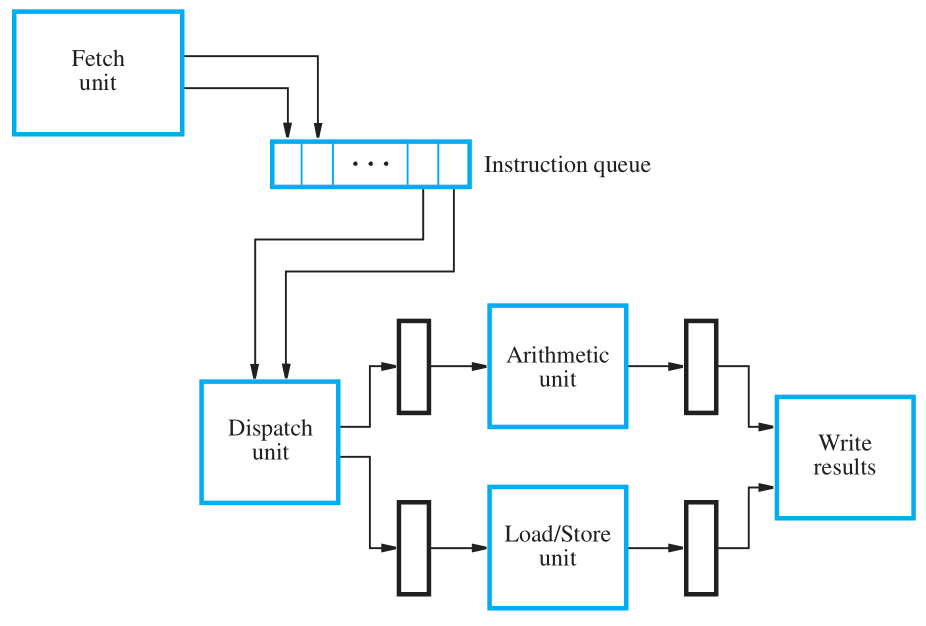
\includegraphics[width=7.8cm]{basic_architecture.PNG}
	\caption{Basic structure of the implemented processor \cite{Hamacher}}
	\label{fig:basic_arch}
\end{figure}

\section{Implementation}

The implemented processor follows the architecture depicted in Figure~\ref{fig:basic_arch}. Thus, it features a Harvard architecture with a four stage pipeline (Fetch, Dispatch, Execute, Write Back) with an ALU and a load/store unit in parallel in the execution stage. In order to utilise the parallel execution units, two instructions per cycle are fetched, enqueued, dequeued and dispatched respectively. The whole design was implemented using the \emph{Chisel} hardware description language.

%# TODO move?
As the evaluation of the processor was conducted with rather simple single-threaded programs (cf. Section~\ref{sec:eval}), the following instructions were not implemented and thus interpreted as NOP: FENCE, ECALL, EBREAK. Otherwise, \emph{A Little Riscy} is except for some memory limitations (cf. Section~\ref{sec:memory}) compliant with the RV32I instruction set.


\subsection{Fetch Unit}
The fetch unit loads two instructions per cycle from the instruction memory and places them into the instruction queue. Additionally, it administrates the PC. In case the queue is full, the whole fetching process is stalled.

Furthermore, it implements all control flow transfer instructions. This implies the following:
\begin{itemize}
	\item As there is no ALU in a previous pipeline stage, additional hardware is required for address calculations.
	\item To ensure the correct register values are present while calculating addresses, the fetch unit has to wait for all previous instructions to take effect before the calculation. This implies that no instructions can be queued until the whole pipeline is idle.
\end{itemize}

The latter can in principle be mitigated using branch prediction an speculative execution techniques, however this was outside the scope of this project.

\subsection{Instruction Queue}
The instruction queue is a simple register based FIFO (cf. the \verb|RegFifo| in \cite{schoeberl}) with a width of $96$~bits ($2\times32$~bits instruction, $32$~bits PC). This brings the limitation that only the two instructions being enqueued together can be dequeued at the same time. In case of structural hazards, this leads to a serialised processing.

\subsection{Dispatcher}
% Details & Discussion Dispatcher (why no Tomasulo?)

\subsection{Execution Units}

\subsection{Memory System} \label{sec:memory}
% Instruction and Data, addressing constraints

\section{Evaluation} \label{sec:eval}

%#TODO used test code (in C)

%# TODO used compiler (incl. flags) and rearrangements, used simulation environment

%# TODO results in tabular form

\begin{table} [h]
	\caption{}
	\centering
	\begin{tabular}{l c}
			Benchmark & IPC \\
		\midrule
			xx & yy\\
	\end{tabular}
	
	
	\label{tab:results}
\end{table}

%# TODO discussion of results

%# TODO FPGA evaluation, resource consumption
An Altera DE2-115 evaluation board featuring an Altera Cyclone IV FPGA was used for evaluation.

\section{Conclusion and Outlook}

%# TODO recap 

%# TODO summary of results, limitations

%# TODO discussion of conceivable extensions to mitigate limitations
\cite{HP}


\printbibliography

\end{document}